%%%%%%%%%%%%%%%%%%%%%%%%%%%%%%%%%
% 6CCS3PRJ Final Year Individual Project Report
% luke.day@kcl.ac.uk
%%%%%%%%%%%%%%%%%%%%%%%%%%%%%%%%%
\documentclass[11pt]{informatics-report}
\usepackage{mathtools}
\usepackage{color}
\usepackage[square,sort,comma,numbers]{natbib}
\usepackage{listings} %References
\usepackage{semantic}
\usepackage{fancyvrb}

%%%%%%%%%%%%%%%%%%%%%%%%%%%%%%%%%
% Front Matter - project title, name, supervisor name and date
%%%%%%%%%%%%%%%%%%%%%%%%%%%%%%%%%
\title{6CCS3PRJ Final Year\\\vspace{0.2cm}Lispish to JavaScript compilation}
\author{Daniel Marian Zurawski}
\studentID{1015180}
\supervisor{Christian Urban}

\date{16th November 2012}

\abstractFile{FrontMatter/abstract.tex}
\ackFile{FrontMatter/acknowledgements.tex} %Remove line if you do not want acknowledgements

\begin{document}
\createFrontMatter
\onehalfspacing
\tableofcontents
\doublespacing

%%%%%%%%%%%%%%%%%%%%%%%%%%%%%%%%%
% Report Content
%%%%%%%%%%%%%%%%%%%%%%%%%%%%%%%%%
% You can write each chapter directly here or in a separate .tex file and use the include command.

\chapter{Introduction}
"This is one of the most important components of the report. It should begin with a clear statement of what the project is about so that the nature and scope of the project can be understood by a lay reader. It should summarise everything that you set out to achieve, provide a clear summary of the project's background and relevance to other work, and give pointers to the remaining sections of the report, which will contain the bulk of the technical material"  .... \\
Following the invention of high performance JavaScript compilers such as the Google V8 JavaScript Engine, raised the interest in creating programming language interpreters and compilers that target JavaScript. It enables applications written in other languages, very often higher level languages to be run on any modern web browser. \\
 
 \section{Motivation}
There are two categories of motivations behind this project. The first category is strictly practical and covers the engineering aspects of this project and the second category is strictly theoretical, as it uncovers an unexplored problem in computer science. In the sub sections below, I would like to introduce these motivations:

\subsection{Theoretical}
I am going to investigate an implementation of a translator that allows for a programming paradigm shift. The translator is going to compile a functional language to an imperative language. 

Preceeding the implementation of the translator, I will have to design a small Lisp based language called Lispish and I will investigate how it can be translated to an executable JavaScript. Lispish is going to implement a subset of the Clojure programming language.

From an engineering perspective, Lispish will provide a way to write programs in Lisp, that can execute in any modern web browser. Lispish could also allow for simple interaction with the DOM elements of web pages, as long as any arbitrary JavaScript function call can be invoked from within Lispish.
One of the practical aspect of this project will also involve investigating how a functional Lisp language can be used for compilation, as the implementation language that will be used to implement the compiler will be Clojure, which is a modern dialect of Lisp running on the JVM.  

This project offers a good opportunity to deepen understanding of functional programming using Lisp and JavaScript and how both can be used to solve complex problems in Computer Science. 

As there already exists a number of similar projects that target JavaScript, I will investigate how each compares to my Lispish to JavaScript compiler.

\section{Report Structure}
Chapter 2 will provide the background research and rationale behind this project. \
Section 2.1 of chapter 2 aims to explain the differences between functional and imperative programming paradigms. 
Section 2.2 goes into the details of the two main programming languages involved in the project, namely Clojure and JavaScript and tries to summarise the differences and similarities of each. 
Section 2.3 briefly explains the reasoning for choosing JavaScript as a target language for our Lisp language.
Section 2.4 introduces the different existing implementations of Lisp to JavaScript compilers.

Chapter 3 defines the language of Lispish and describes the compilation pipeline.
Chapter 4 describes the test suite and showcases the functioning compiler using test cases as examples

\listoffigures

\chapter{Background}
This section provides throughout background research of the domain of functional programming, Lisp and JavaScript that lead me to the rational behind Lispish design decisions. 

It also covers existing implementations of Lisp to JavaScript translators and covers the professional issues that need to be taken into consideration in this project. 

\section{Bridging the gap between functional and imperative paradigm}

\subsection{Functional and imperative paradigms comparison}
Functional programming is a programming paradigm that differs from imperative programming in a way that it focuses solely on evaluating functions, where one input always results in the same output for a given input (referential transparency). In imperative programming, this notion is not always true, as imperative programming focuses a lot more on modifying the state of the application as it runs. To make referential transparency, pure functional languages try to avoid using state and mutability, by ensuring that side effects that could introduce state changes are not possible.

An example of state is preserving results in variables for later access by other parts of the program. A side effect may result from many different operations such as variable assignments, input or output operations and anything that allows two parts of the program to access the same resource at the same time.

Due to the increase of the demand for parallelisation, as more processing cores are added to modern CPUs, it is therefore essential that the software we write can be parallelised easily and without the risk of errors that could be caused by race conditions or deadlocks - which are all caused by the notion of mutability that is present in imperative languages.

The notion of pure functions may sound very impractical for a general purpose programming language, therefore functional languages used by practitioners such as Clojure allow state, but lexically scoped to its own function.
When state is absolutely necessary in order to improve the performance of an application or expose variable to other parts of the program, Clojure allows for so called "atoms", that improve on the classical notion of a variable, as it is still immutable, but instead an atomic swap operation of the content is performed whenever want to override the original state.

The property of immutability is also preserved for data structures, as each time a data structure is modified, a new copy of such structure is retained therefore leaving the old one in tact. This allows for much better parallelisation, as one part of the program may never modify the same data as the other part of the program, which would lead to inconsistent state.

\section{Programming languages involved}
In order to complete this project, it is necessary not only to understand the two different programming paradigms, but also the specific features of each of the languages involved - Clojure and JavaScript.
We will use Clojure as an example of a functional language, as Lispish is a subset of Clojure and the compiler itself is also programmed in Clojure.

\subsection{Clojure}
Clojure~\cite{Clojure:2013:Site} is a functional language, which is implemented as a dialect of Lisp and primarily targets the Java Virtual Machine. It can also target Microsoft's Common Language Runtime, which is the virtual machine for the .NET Framework through Clojure's sub-project \textbf{clojure-clr}~\cite{clojure-clr}. 
It also targets JavaScript by means of \texttt{ClojureScript}~\cite{ClojureScript:2013:Site}, which is a subset of Clojure that compiles to JavaScript. 

Clojure is a powerful abstraction over standard Java, which as of today does not provide lambdas and any of the functional constructs that Clojure does, including immutability and treating code as data.

\subsubsection{Lisp}

Lisp is amongst one of the worlds oldest family of programming languages, that has developed several dialects since the original Lisp was published in 1958-1960 by John McCarthy. [citation here]
Lisp languages differ from other programming languages 
% TODO grammar 'in its'
in its few original concepts, notably treating code as data, s-expressions, parenthesized Polish prefix notation and lambda expressions.

The exact expansion of the Lisp acronym is List Processing, which has its practical reasons -- Lisp source code is written as lists, formally known as S-expressions~\cite{s-expression}\cite{s-expression-wiki}.

To illustrate how a valid s-expression would look like compared to an equivalent Java expression, figure~\ref{fig:norvig-lisp-comparison} shows an excerpt from Peter Norvig's \textit{A Retrospective on Paradigms of AI Programming}~\cite{retrospective.norvig}. The figure illustrates the comparison of complexity in defining a lambda function in Lisp and in Java. 
As we can see, Lisp is not only a lot clearer syntactically, but it is also shorter and accomplishes the same goal.  

\begin{figure}[ht]

\begin{quote}
"[...] Java has anonymous classes, which serve some of the purposes of closures, although in a less versatile way with a more clumsy syntax. In Lisp, we can say \texttt{(lambda (x) (f (g x)))} where in Java we would have to say

\begin{verbatim}

new UnaryFunction() { 
  public Object execute(Object x) {
    return (Cast x).g().f();
  }
}
\end{verbatim}
where Cast is the real type of x. This would only work with classes that observe the UnaryFunction interface (which comes from JGL and is not built-in to Java). [...]"
\end{quote}

\caption{Excerpt from Peter Norvig's \textit{Paradigms of Artificial Intelligence Programming: Case Studies in Common Lisp}. Comparison of a Lisp and Java lambda function declaration.\cite{PAIP.Norvig}}
\label{fig:norvig-lisp-comparison}
\end{figure}


The article also shows an interesting view on the recent advancements of other languages compared to the ancient Lisp and it's a retrospective to the \textit{Paradigms of Artificial Intelligence Programming: Case Studies in Common Lisp}~\cite{PAIP.Norvig}. This is Peter Norvig's book about Aritficial Intelligence where all of the examples have been programmed in Common Lisp.

The simplicity and conciseness of Lisp syntax has been the main motivating factor to choose Clojure (being a functional language of the Lisp dialect) as the basis for the Lispish language. 

\subsubsection{Portability}
Due to the fact that Clojure targets the Java Virtual Machine, programs written in this language can be executed in any environment where the Java Runtime Environment is installed by means of executing Clojure programs packaged as JAR files, given that they have been packaged to include Clojure itself.  

Clojure programs can co-operate with Java applications due to its great interoperability. They can be imported into Java programs as aforementioned JAR files.

Clojure can also access all of the core Java static classes/methods, making it a very powerful abstraction over Java. It is not only because it's a very portable functional language that works with immutable data structures, but also because it gives access to the wealth of Java libraries and the entire JVM eco-system.

\subsection{JavaScript}
JavaScript is an interpreted, dynamically typed, prototyped, functional programming language that originated from the ECMAScript language in 1995. It was originally intended as a client side scripting language for web browsers, but it has since evolved to an extent where well-known corporations such as Microsoft support it as a language of choice for deploying web applications on their cloud-service offerings \cite{nodejs.WindowsAzure}. This is due to its rich support for multiple programming styles, including functional programming. More on this below in section ~\ref{portability} (JavaScript: Portability).  

\subsubsection{JavaScript Performance}
The creation of the V8 Google JavaScript Engine made JavaScript stand out from other dynamic languages by making it significantly faster than for e.g. Python ~\cite{JavaScriptVSPython3} or Ruby ~\cite{JavaScriptVSRuby}.

Due to the fact that Lispish compiles to JavaScript, the generated code can be treated with various optimisation techniques (such as the Google Closure compiler that minimises and optimises the code) by compiling the human-readable to unreadable but highly optimised JS code.

\subsubsection{Portability}\label{portability}
JavaScript interpreters are present on majority of consumer devices and are present in all of the modern web browsers. It is the basis of Rich Internet Applications and is now not only present on the front-end of the web browser, but also serves as a language of choice on the server-side.

Most notable examples include Microsoft's adoption of \texttt{node.js} for their cloud platform Windows Azure ~\cite{nodejs.WindowsAzure}, as the basis for producing highly concurrent web applications. It enables developers to write server-side applications that operate using JavaScript both on the front-end and back-end using a single programming language.

\subsection{Compiling Lispish Using a Dialect of Lisp}
The decision to use Clojure to write a compiler for my Lisp language comes from the fact that there are large advantages to using Lisp to compile Lisp.
% TODO reference for above
The nature of Lisp and its s-expressions allow us to build efficient recursive descent parsers that can take advantage of already present functions in our implementation language, Clojure.

There is a number of complexities that we would encounter when trying to implement a Lisp compiler using a non-Lisp imperative language such as C.
These include having to determine if a given expression is an s-expression (list) or a symbol, breaking the input down into its atomic form of tokens, building a Parse Tree (ST) or an Annotated Syntax Tree (AST).
In our case, our input s-expressions in their prefix notations can be treated as a parse tree and thanks to the in-built functions we can greatly simplify the compiler.

For example, any s-expression can be essentially type-checked using the in-built \texttt{(symbol? )} or \texttt{(list? )} to determine if the given s-expression yields a symbol or a list of expressions. If an input is a list, that means we have encountered another s-expression and each element in the list has to be separately evaluated.

Modern dialects of Lisp, such as Clojure, target the Java Virtual Machine making them very portable and pluggable into an existing Java applications.
Other Lisp languages are very often compiled to another target language, such as C or JavaScript that can be then run on a variety of machines. Notable examples of Lisp to C compilers include Stalin \cite{stalin} (STAtic Language ImplementatioN) and Chicken \cite{chicken}. 

\section{JavaScript as the Target Language for the Lispish Language}
The rationale behind selecting JavaScript as the target language is the fact that JavaScript can be executed on almost all Internet-enabled devices.

Our small dialect of Lisp (Lispish) language will allow generating pluggable JavaScript code.
From this follows that applications written in Lispish can be executed in environments where the JVM or Clojure is not present as the generated code will be standard JavaScript.
In theory, our language could even be used as a Domain Specific Language (DSL) for JavaScript applications, as long as the code would be evaluated by our compiler in a Clojure JVM environment.

JavaScript offers a great opportunity as a target language for any high-level programming language primarily due to two reasons - its portability and performance.

\subsection{Similarities}
Similarly to other Lisp languages, JavaScript supports the functional paradigm and provides full support for lambda expressions. It also provides a great deal of flexibility with its support for prototype-based object-orientation which could be compared to Lisp macros used for extending the language.

\begin{figure}[ht]
\begin{verbatim}
// Attach event listener to the argument
var assign-event-listener = function(x) {
  x.addEventListener("load", function() {
    alert("All done");
  }, false)
};
\end{verbatim}
\caption{JavaScript event listener function}
\label{fig:js-attach-event-listener}
\end{figure}

Figure~\ref{fig:js-attach-event-listener} illustrates a stored function that takes a reference to a web browser's window as an argument and attaches an event listener to it. The listener then takes two arguments, a string describing the event (here "load") and the callback function (here an anonymous function that displays an alert "All done") that gets displayed when the desired event is triggered.

\begin{figure}[ht]
\begin{verbatim}
(defn assign-event-listener [window]
	"Attach event listener to the argument"
	(window (addEventListener
            	"load"
                (fn [x] (alert "All done")))))
\end{verbatim}	
\caption{Possible Lisp equivalent of event listener function}
\label{fig:lispish-attach-event-listener}
\end{figure}

Similarly, the equivalent expressions written in Lisp could look like on figure ~\ref{fig:lispish-attach-event-listener}, which is arguably a lot more readable. Nonetheless, both expressions look alike. 

Both expressions make use of nested functions and thus, take advantage of lambda calculus. 

As lambda functions are inherent to programming applications in a functional language, the design and implementation of the translator will make an extensive use of lambda functions.

\section{Existing Lisp to JS Compilers}\label{existing-implementations}
% TODO
There already exists a number of similar projects, each of which tries to solve the problem in a slightly different way. Nevertheless, there exists only one mature compiler that can actually generate an executable JavaScript code and it is called ClojureScript.

\subsection{ClojureScript}
ClojureScript~\cite{ClojureScript:2013:Site} is a Clojure to JavaScript compiler that generates code that can be executed in the browser. Although there are examples of companies using ClojureScript for their production applications, it is difficult to operate as it requires to execute a chain of operations, including starting a JavaScript program before the Clojure code can be compiled.

ClojureScript also takes the idea further and utilises the Google Closure compiler to optimise the code but this approach suffers from the possibility of breaking the JavaScript code that was compiled from Clojure. However, the ClojureScript project page claims, that the JavaScript generated is compatible with the \texttt{advanced} mode of the Google Closure compiler.

% TODO
ClojureScript is a production ready project and has been deployed numerous times in production environment. It is also the official 

\subsection{Outlet}
Outlet~\cite{Outlet:2013:Site} is a Lisp-like programming language that compiles to JavaScript. Its compilation is interesting in that the compiler itself is written in Outlet, only after it is bootstrapped by a JavaScript interpreter.
The bootstrapping interpreter is implemented using grammar rules similar to Backus-Naur Form context-free grammars ~\cite{RecursiveDescentParserJS:2013:Site}, thus ensuring that the initial interpretation of the main constructs is correct. This approach provides a solid foundation for then implementing rest of the constructs of the Outlet language, in Outlet.

Outlet does not provide the ability to define macros, thus there is no way to dynamically extend the language without modifying the compilers source, which is a big feature of a Lisp language.

\subsection{LiScript}
LiScript~\cite{LiScript:2013:Site} is yet another Lisp language that compiles to JavaScript. It supports roughly 20 forms, 13 of which replace the regular binary and arithmetic operations of \texttt{$>$}, \texttt{$<$} etc. and the remaining 7 are forms such as \texttt{if}, anonymous function \texttt{fn} and iterating constructs such as \texttt{iter} and \texttt{while}.

LiScript is implemented in JavaScript and it is surprisingly lightweight. The entire implementation is around 100 lines of code. Nonetheless, it can generate a readable and, most importantly, executable JavaScript code. 

LiScript allows defining new language constructs by means of macros, a special form \texttt{defmacro}. This allows for building new forms from arbitrary strings, as input to the defmacro form first modifies the code and only then evaluates it. 

\subsection{clojurejs}
ClojureJS~\cite{ClojureJS:2011:Site} is a small subset of Clojure to JavaScript compiler.
ClojureJS takes on an approach different to the preceding implementations, as the compiler is written in Clojure. 
It is a hand-written recursive descent parser that requires a running Clojure environment in order to evaluate input source code, which is of the form of a subset of Clojure.

% TODO
ClojureJS is perhaps the second best implementation of Clojure to JavaScript compilation, with its support for macros and a lot larger subset of Clojure than, for instance, LiScript. 
It is, however, a non-extensible implementation of a trans-compiler and it does not provide any ease-of-use features, such as being able to generate an output \texttt{.js} file out of a given source input. 

\section{Professional and ethical issues}
Throughout the report, I will make sure that I am not violating the British Computer Society Code of Conduct and Code of Good Practice and that I have applied their principles throughout the project.

All possible efforts shall be made to properly state and reference communicating someone else's ideas.

\chapter{Design \& Specification}

As previously described, the project aims to create an extensible Lispish to JavaScript compiler. 
In order to ... we need to formalise our input language Lispish to clearly define the possible constructs that we allow in our program. 
As Lispish defines a subset of an existing language, it is therefore even more important to be clear on what it possible and what is not. 

\section{Designing the Lispish language}

Lispish is a dynamically typed, functional language that implements a call-by-value strategy just as its superset Clojure.

The formal description of Lispish behaviour will be described using transition systems.

\subsection{Grammar of Lispish}

$F \Coloneqq \ (let \ [x \ F] \ (F)) \\
| \	(if \ (F) \ F_1 \ F_2) \\
| \	(defn \ name \ [args*] \ (F)) \\
| \	(fn \ [arg] \ (F)) \\
| \	(cond \ (F_0) \ F_1 \ (F_2) \ F_3) \\
| \     T \\
| \     X
$

where
\\
$X \Coloneqq T $
\\
$T \Coloneqq \ () \ \vert \ N \ \vert \ B \ \vert \ s $
\\
$N \Coloneqq n \ \vert \ (op \ N \ N)  $
\\
$B \Coloneqq b\ \vert \ (bop \ t1 \ t2) \ $
\\
$op \Coloneqq \ + \ \vert \ - \ \vert \ * \ \vert \ /$
\\
$bop \Coloneqq \ > \vert < \vert =$
\\
$s \Coloneqq \ String $
\\
$n \Coloneqq \ Integer $
\\
$b \Coloneqq \ true \ \vert \ false $
\\
$() \Coloneqq \ List $

\subsection{Evaluation relations (Big-Step Semantics)}
Operators:
\[
\inference[bop]{E_1, s \ $$\Downarrow$$ \ b_1, s' \ E_2, s' \ $$\Downarrow$$ \ b_2, s''}
{(bop \ E_1 \ E_2) \ $$\Downarrow$$ \ b, s'', if (= b \ (bop \ b_1 \ b_2))}
\]
\[
\inference[op]{E_1, s \ $$\Downarrow$$ \ n_1, s' \ E_2, s' \ $$\Downarrow$$ \ n_2, s''}
{(op \ E_1 \ E_2) \ $$\Downarrow$$ \ b, s'', if (= b \ (op \ n_1 \ n_2))}
\]


Atomic:

\[
\inference[String]{}
{s \ $$\Downarrow$$ \ s}
\]
\[
\inference[Integer]{}
{n \ $$\Downarrow$$ \ n}
\]
\[
\inference[List]{n \ $$\Downarrow$$ \ v}
{(n) \ $$\Downarrow$$ \ v}
\]
Forms (F):
\[
\inference[let]{t_0 \ $$\Downarrow$$ \ v}
{(\text{let } \ {[x \ (t_0)]} \ (t_1)) \ $$\Downarrow$$ \ t_1 {[}x \ $$\mapsto$$ \ v{]} }
\]
\[
\inference[if true]{{t_0} \ $$\Downarrow$$ \ \textsc{True} & t_1 \ $$\Downarrow$$ \ v}
{(if \ (t_0) \ t_1 \ t_2) \ $$\Downarrow$$ \ v) }
\]
\[
\inference[if false]{t_0 \ $$\Downarrow$$ \ \textsc{False} & t2 \ $$\Downarrow$$ \ v}
{(if \ (t_0) \ t_1 \ t_2) \ $$\Downarrow$$ \ v) }
\]
\[
\inference[cond]{t_0 \ $$\Downarrow$$ \ \textsc{False} & t_1 \ $$\Downarrow$$ \ \textsc{True} & t_3 \ $$\Downarrow$$ \ v}
{(cond \ (t_0) \ t_2 \ (t_1) \ t_3) \ $$\Downarrow$$ \ v) }
\]
\[
\inference[defn]{ {t_0 \ [x]} \ $$\Downarrow$$ \ v}
{(defn \ s \ {[x]} \ (t_0)) \ $$\Downarrow$$ \ s \ $$\mapsto$$ \ v }
\]
\[
\inference[fn]{ {t_0 \ [x]} \ $$\Downarrow$$ \ v}
{(fn \ {[x]}  \ (t_0) \ $$\Downarrow$$ \ v }
\]

\section{Development methodology}
In order to streamline the process of development of the compiler, I have decided to use the Test Driven Development (TDD) methodology that emphasizes on building small units of functionalities that can be invidually tested by individually unit tests. 

Clojure allows developers to create programs using the REPL (Read Evaluation Print Loop), which is characteristic feature in new dynamic programming languages. It allows you to write your functions, evaluate them and get an instant result from an interpreter that interacts with your code. This in essence reduces the amount of unit tests that have to be implemented for trivial functions in a TDD project. 
REPL is a great resource for rapid development and prototyping of functions, but also ensuring that they yield the right result before the project as a whole is compiled.

\subsection{Unit tests}
Even though Clojure provides REPL, it is still important to develop a regression testing suite that ensures whenever the compiler is modified, it can still compile and yield the same result for old programs.
To do this, I will use clojure.test API that provides a set of macros for evaluating forms and ensuring they yield the expected result. 

\section{Compiling Lispish to JavaScript (Compiler design??)}

\subsection{Compilation pipeline (use case/state machines?)}

\begin{figure}[hb]
	\centering
	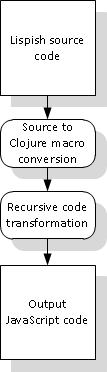
\includegraphics{Graphics/test.jpg}
	\caption[Abstract \textit{Lispish to JavaScript} compilation.]
   {Abstract figure of \textit{Lispish to JavaScript} compilation.}
\end{figure}

The compiler in its simplest form will perform a one to one translation in-line translation from Lispish to JavaScript. 
The input source will be treated by a macro function that will prevent the code from being evaluated and it will pass it along down the pipeline to its respective emitters as ilustrated on figure ~\ref{fig:abstract_compilation}. Code will be treated as data and I will use the prefix notation to my advantage, treating each expression as its respective node in a parse tree. 

\subsection{Alternative approach}

\chapter{Implementation and Testing}

\section{Section Heading}
\chapter{Professional Issues}
Either in a separate section or throughout the report demonstrate that you are aware of the \textbf{Code of Conduct \& Code of Good Practice} issued by the British Computer Society and have applied their principles, where appropriate, as you carried out your project.

\section{Section Heading}
\chapter{Results/Evaluation}
The implementation of Lispish to JavaScript was supposed to serve as an example of how in a simple way, a programming language translator can be implemented.

Due to its functional nature and immutability, it does not suffer from errors caused by inconsistent state, as there is no state. The compiler will always produce a result. The result however is not guaranteed to be correct, if an incorect input has been provided. 

Appendix [REFERENCE HERE] provides a set of unit tests that include three real applications of our translator by translating a Clojure Fibonacci, factorial and Ackermann functions to its equivalent JavaScript functions, as well as smaller tests that check the correctnes of single forms.
The unit tests included in the above mentioned appendix all successfully pass.
The compiler also successfully compiles a given input file to an output file with name of our choice. 

\section{Missing parts}
\subsection{Error handling}
The compiler does not provide any facility for error reporting during the compilation.

The compiler does not have any means of validating the JavaScript code. This could be incorporated by means of bundling a JavaScript validator that could simply analyse the code before it's served to an output file. This was however not part of the initial design and due to time constraints has not been implemented.

The biggest issue with the compiler is that it does not actually parse the input string before the compilation is performed. This caveat removes the posibility of determining if the input source, that is Lispish, is actually valid. 
Providing an invalid Lispish source code would still result in a JavaScript output, but the generated code would be malformed and would not execute in a browser. This is both true for semantical, as well as syntactical errors.

\section{Future work}
\subsection{Parser}
In order for Lispish translator to be a true compiler, it would need a parser that can decide whether the input string, that is the Lispish program, is in fact a correct one. As mentioend in the section above, it does not provide any error detection facility and this therefore would be the first step for proper error handling. 
\subsection{JavaScript validator}
For Lispish to be trully useful, its translator would have to have a JavaScript validator in place. 
JavaScript that is not syntactically correct due to the faulty input Lispish is only going to decrease the productivity of the developer, which goes against the core idea of building an abstraction over an imperative language.

\chapter{Conclusions and Future Work}

Functional compilers provide an elegant alternative to compilers written in imperative languages. Nevertheless, it is not trivial to implement one given the relative unpopularity of functional programs. 

The translator in its current state could be a good foundation for initiating a collaboration with the open source community that could have interest in extending it. 

It was not in the scope of this project to provide any formal proofs of the correctness of the translations. This, however, would be a very achievable target, mainly due the functional properties of the compiler -- namely the one-input/one-output property. 
Providing formal proofs for the correctness of the translator and even further, of the generated translations could be a good project for a Master's Thesis. 

\section{Future work}
\subsection{Macros}
It is typical for Lisp languages to provide a way to define new constructs in terms of already existing language constructs.
For this to happen, a language needs to support macros which 
provide a way to extend the language at compile time. 
Due to time constraints, I was unable to perform sufficient research into how to provide the flexibility of macros, while still being able to parse the code correctly. 

\subsection{Parser}
In order for the Lispish translator to be a true compiler, it would need a parser that can decide whether the input string, that is the Lispish program, is in fact valid. As mentioned in the previous chapter, the current compiler does not provide any error detection facilities and this therefore, would be the first step to proper error handling. 

\subsection{Supporting a Greater Subset of Clojure}
Lispish implements a fair subset of Clojure. Adding support for a bigger subset
(if not the entirety of the language) is a reasonable next step should further development occur. This would be facilitated by the project's design which allows for extending the functionality in this respect.

\subsection{Code Optimisation}
One possible improvement, that was outside of the scope of this project, would be to optimise the input that the compiler receives before transforming it into JavaScript. Possible optimisations could include removing dead code and  computing the value of constant expressions.

\subsection{JavaScript Strict Mode Compliance}
Due to the use of the \texttt{arguments.callee} function used to facilitate the implementation of the \texttt{(recur )} form (see the relevant implementation section \ref{arguments.callee} on page \pageref{arguments.callee}), the compiler's output is not Strict mode compliant and thus, might not run should that be enabled.
Creating an alternative solution that would bring the output code into compliance would be a worthwhile pursuit.


%%%%%%%%%%%%%%%%%%%%%%%%%%%%%%%%%
% References
%%%%%%%%%%%%%%%%%%%%%%%%%%%%%%%%%
\bibliographystyle{plain}
\bibliography{references}
\addcontentsline{toc}{section}{Bibliography}

%%%%%%%%%%%%%%%%%%%%%%%%%%%%%%%%%
% Appendices
%%%%%%%%%%%%%%%%%%%%%%%%%%%%%%%%%
\appendix
\include{Appendices/appendix}
\chapter{User Guide}
\section{Instructions}
You must provide an adequate user guide for your software. The guide should provide easily understood instructions on how to use your software. A particularly useful approach is to treat the user guide as a walk-through of a typical session, or set of sessions, which collectively display all of the features of your package. Technical details of how the package works are rarely required. Keep the guide concise and simple. The extensive use of diagrams, illustrating the package in action, can often be particularly helpful. The user guide is sometimes included as a chapter in the main body of the report, but is often better included in an appendix to the main report.

\chapter{Source Code}
\section{Instructions}

I verify that I am the sole author of the programs contained in this folder, except where explicitly stated to the contrary.
-- Daniel Zurawski, 17 April 2013.

\subsection{lispish/project.clj}

\begin{verbatim}
(defproject ClojureToJavaScript "1.0.0-SNAPSHOT"
  :description "FIXME: write description"
  :dependencies [[org.clojure/clojure "1.3.0"]
                 [org.clojure/tools.trace "0.7.3"]
                 [org.clojure/tools.cli "0.2.1"]]
  :main lispish.core)
\end{verbatim}


\subsection{lispish/src/lispish/core.clj}

\begin{verbatim}
(ns #^{:author "Daniel Zurawski"
       :doc "A simple Lisp to JavaScript transcompiler written in Clojure."}
  lispish.core
  [:require
   [clojure.string :as str]]
  [:use
   [clojure.walk]
   [clojure.tools.trace]
   [clojure.tools.cli :only (cli)]]
  (:gen-class :main true))


(def op (set ['mod '+ '- '* '/ '> '< '=]))
(def bop (set ['or 'and 'not]))
(def forms (set ['recur 'let 'if 'fn 'defn 'cond]))

;; Clojure is a single pass compiler, thus we have to use forward declaration
;; if we need to use a function before it's declared
(declare emit-list)

(defn emit [expressions]
  "Take an s-expression and emit its corresponding JavaScript form"
  (do
    (println "Top level - Emit Lispish: " expressions)
    (cond
      (nil? expressions) "null"
      (symbol? expressions) (str expressions)
      (seq? expressions) (emit-list expressions)
      (integer? expressions) (str expressions)
      (float? expressions) (str expressions)
      (string? expressions) (str \" expressions \")
      :else (str expressions))))

;; Abstract Structural Binding - + falls in type, + in op and 2 2 in tail
(defn emit-op [type [op & tail]]
  "Emit s-expression with single operators and two arguments"
  (do (println "Emit-op, head: " op ", tail: " tail)
      ;; Interlace the arguments with the operator
      (if (= op 'not)
        (str "(!" (emit tail) ")")
        (str "(" (clojure.string/join
                (str (cond (= op '=) "=="
                           (= op 'mod) "%"
                           (= op 'or) "||"
                           (= op 'and) "&&"
                           :else op))
                (map emit tail))
           ")"))))

(defn emit-let [type [let [x y] body]]
  (println "Emit-let, x: " x ", y: " y ", body: " body)
        (str "(function(" (emit x) ") { return "  (emit body)  " })(" (emit y) 
        ")" ))

(defn emit-if [type [if condition true-form & false-form]]
  (println "Emit-if, condition: " condition ", true-form: " true-form ", false-
  form: " false-form)
  (str "("
       (emit condition)
       " ? ("
       (emit true-form)
       "):("
       (emit false-form)
       "))"))

(defn emit-defn [type [defn name [arg & more] & rest]]
  (do
    (println "Emit-defn, name: " ", arg: " arg ", arg tail: " more ", rest: " rest))
  (str (str "function " (if (= "~" name) "" name) "("
            (if (nil? more) arg (str arg ", " (clojure.string/join ", " more)))
             ") {return "
       (emit rest)
       "}")))

(defn emit-fn [head expression]
  (emit-defn head (concat (take 1 expression) '("~") (drop 1 expression))))

(defn emit-call [head [name args & rest]]
  (println "Emit-call, name: " name ", args: " args ", rest: " rest)
  (str name "("
       (if (nil? rest)
         (str "(" (emit args) ")")
         (str (str (emit args)) ", " (clojure.string/join ", " (map emit rest))
         )) ")"))

(defn emit-recur [head expression]
  (println "Emit recur, head: " head ", expression: " expression)
  (emit-call head (concat '("arguments.callee") (drop 1 expression))))

(defn emit-cond [head [name & rest]]
  (let [rev (reverse (partition 2 rest))]
    (println "Emit-cond, head: " head ", name: " name ", rest: " rest 
    ", reverse after partitioning: " rev)
    (reduce
          (fn [a b] (do (println "a: " a ", b: " b ) (str "(" (emit (first b)) 
          "?" (emit (second b)) ":" a ")")) )
          (str (emit (second (first rev))))
          (drop 1 rev))))

(defn emit-forms [head expression]
  (do (println "Emit-forms, head: " head ", full expression: " expression)
      (cond (= head 'let) (emit-let head expression)
            (= head 'if) (emit-if head expression)
            (= head 'fn) (emit-fn head expression)
            (= head 'defn) (emit-defn head expression)
            (= head 'cond) (emit-cond head expression)
            (= head 'recur) (emit-recur head expression)
            :else (emit-call head expression) )))

(defn emit-list [expressions]
  (do
      (if (symbol? (first expressions))

        (let [head (symbol (first expressions))
              expressions (conj
                           (rest expressions) head)]

          (println "Emit-list head: " head
                   ", tail: " (rest expressions))
          (cond
            (or (contains? op head) (contains? bop head)) (emit-op head expressions)
            (contains? forms head) (emit-forms head expressions)

            :else (emit-forms head expressions)
            ))
        ;; Not safe, may run into stack overflow if this will be a list or not-
        recognized
        (emit (first expressions)))))

(defn lisp-to-js [forms]
  (let [code (read-string forms)]
    (println code)
    (emit code)))

(defn read-file-emit [st file-out]
    (let [form (read st false "")]
      (if (not (= form ""))
        (do
          (spit file-out (str (emit form) "\n")  :append true)
          (read-file-emit st file-out)))))

(defn read-file [file-in file-out]
  (with-open [r (java.io.PushbackReader.
                 (clojure.java.io/reader file-in))]
    (binding [*read-eval* false]
      (spit file-out "" :append false)
      (read-file-emit r file-out))))

(defn run
  "Print out the options and the arguments"
  [opts args]
  (cond
    (:input opts) (if (:output opts)
                    (read-file (:input opts) (:output opts))
                    (println "Please provide --output or -out, path where the output JavaScript file will be generated."))
    (seq args)    (println (lisp-to-js (first args)))
    :else         (println "No path to input source code specified and no code given as argument.")))

(defn -main [& args]
  (let [[opts args banner]
        (cli args
             ["-h" "--help" "Show help" :flag true :default false]
             ["-in" "--input" "REQUIRED: Path to Lispish source code."]
             ["-out" "--output" "OPTIONAL: Path to JavaScript output file."]
             )]
    (when (:help opts)
      (println banner)
      (System/exit 0))
    (if (or (:input opts) (seq args))
      (run opts args)
      (println banner))))
\end{verbatim}
\end{document}
